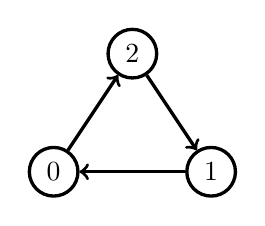
\begin{tikzpicture}[scale=1, line width=1.2pt]
    % \node at (-1.5,1.8) {\Large \(H\)};

    \node[circle, draw=black, fill=white, minimum size=0.05cm] (v0) at (-1,1) {\(0\)};
    \node[circle, draw=black, fill=white, minimum size=0.05cm] (v1) at (1,1) {\(1\)};
    \node[circle, draw=black, fill=white, minimum size=0.05cm] (v2) at (0,2.5) {\(2\)};

    \draw[->] (v0) -- (v2);
    \draw[->] (v2) -- (v1);
    \draw[->] (v1) -- (v0);
\end{tikzpicture}
